% !TEX root = ../main.tex

\chapter{绪论}

\section{研究背景和意义}

医疗图像分割技术是计算机视觉和模式识别技术应用在诸如X-Ray CT(X光计算机断层扫描成像)、MRI(磁共振成像)和Ultrasound(超声成像)等医疗图像上,
针对特定的目标,譬如肺部动脉/静脉血管、乳腺肿块,肺癌结节,进行逐体素(Voxel)的分类。本文聚焦肺部CT扫描图像,研究肺部支气管树状结构的气道分割提取技术。


肺部和呼吸系统疾病对人体健康威胁巨大,自2019年底、2020年初爆发的全球性新冠肺炎COVID-19疫情严重冲击人类的公共卫生与生命健康。三年多来,世界各国在抗击新冠肺炎疫情方面付出了惨重的生命代价和社会经济损失。新型冠状病毒经由空气为媒介传播,通过呼吸道进入肺部并感染细胞。包括肺癌在内的一些肺部疾病,慢性
阻塞性肺疾病(COPD)\cite{fetita2004pulmonary}、急性呼吸窘迫综合症\cite{howling1998significance}、闭塞性细支气管炎\cite{shaw2002role}、特发性肺纤维化\cite{wu2019computed}、肺挫伤\cite{li2019application}等导致肺支气管气道树的形态学变化。
支气管气道树的形态学三维模型通过从基于CT扫描的肺部图像中精确分割出来,是分析包括哮喘、支气管扩张和肺气肿在内的肺部疾病的关键步骤。测量精确分割出来的支气管的气道管腔
尺寸和管壁厚度,可以用于辅助诊断肺栓塞\cite{estepar2013computed}, 揭示慢性阻塞性肺部疾病COPD患者的异常病症。除了上述这些疾病诊断治疗之外,本文研究肺部支气管气道
树分割的一个直接动因是为了开发支气管镜和支气管导航与活体检测的手术机器人。手术机器人驱动细长柔性的支气管镜器械,伸入支气管,沿着气道导航至疑似(肺部)病灶部位,对
病灶处细胞进行活体采样返回,进而化验诊断出疾病。本文作者所在的工作单位就在开发国产的支气管镜导航/检测的手术机器人,而支气管气道树的精确分割就是非常重要的前置研发步骤。
构建出支气管气道树的分割模型后,输入患者的肺部CT扫描图像数据,就可以输出包含精确的三维空间信息的支气管气道树结构。将这个支气管气道树的结构模型“喂给”支气管镜导航机器人
(Bronchoscopy and endobronchical navigation robot),在医生的监视与操纵下,机器人就可以被引导进入支气管管腔内,进行疾病的诊断与治疗了。

{\heiti 支气管气道树的分支结构。} 本文研究支气管气道树的分割,有必要先了解一下支气管数状结构的气道解剖结构。从图\ref{fig:branches_of_bronchial_tree}中可以看出,支气管气道树的分支结构非常复杂,从气管(Trachea)往下分为左、右两支主支气管(Main bronchus),左右两支主支气管各自分岔为上叶支气管(Superior lobar bronchus)、中叶支气管(Middle lobar bronchus)和下叶支气管(Inferior
 lobar bronchus)。在每个肺叶内,起于肺叶的支气管继续分岔为多个肺段支气管(Segmental bronchi)。肺段支气管最后分为更细小的支气管到达肺泡。

\begin{figure}[!htp]
	\centering
	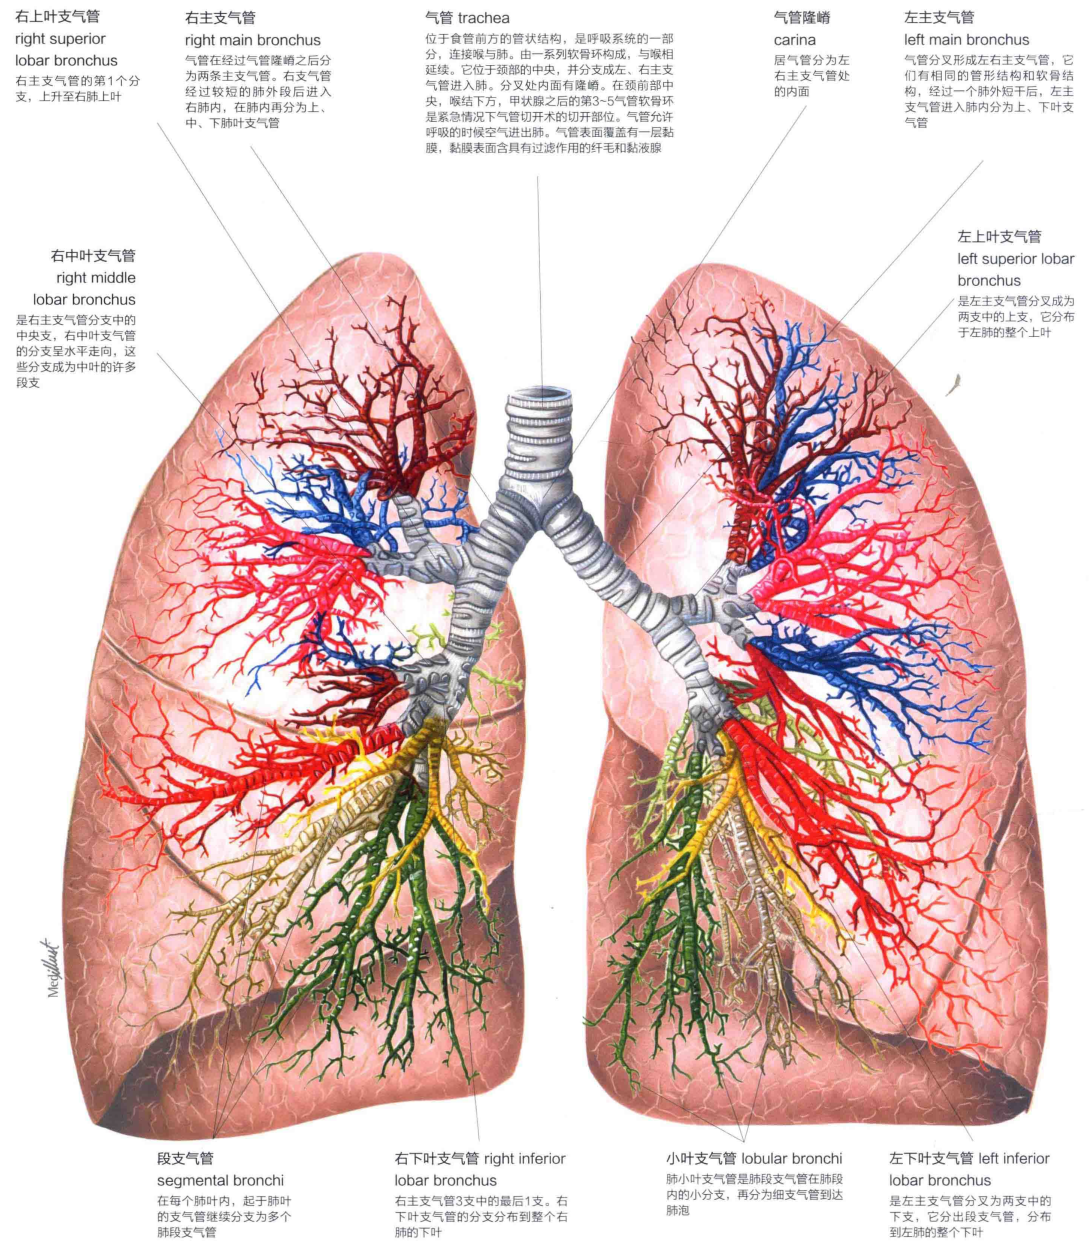
\includegraphics[width=0.9 \textwidth]{branches_of_the_bronchial_tree}
	\bicaption[肺部支气管气道树的分支结构]
		{肺部支气管气道树的分支结构\parencite{humananatomy2nd}}
		{The branch structure of pulmonary bronchial airway tree}
	\label{fig:branches_of_bronchial_tree}	
\end{figure}

如此繁复,从粗到细不断分化,面对如此稠密细小的支气管气道树,进行分割前需要经验丰富的临床专家进行非常细粒度的标注。手工标注耗费大量时间,
成本高昂且支气管越细小,标注越困难,易于出错。 标注任务艰巨繁重,急需开发新的算法或模型来帮助临床医生解决支气管气道树分割的问题。

\section{本研究的应用前景}

肺部支气管气道树的自动化分割是呼吸系统肺部疾病诊断治疗的一个重要问题和研究领域,在实际应用中具有非常重要的作用,提高医疗技术水平。当前,在
作者所在的医疗机器人行业,本研究项目有如下的应用前景:
\begin{itemize}
	\item {\heiti 导管手术机器人 }
	由于肺部支气管气道树三维模型具有精确的空间位置信息,CT扫描建立的坐标系赋予DICOM医疗图像每个像素都有相应的坐标位置信息,如图\ref{fig:coordinate}所示。
	\begin{figure}[!htp]
		\centering
		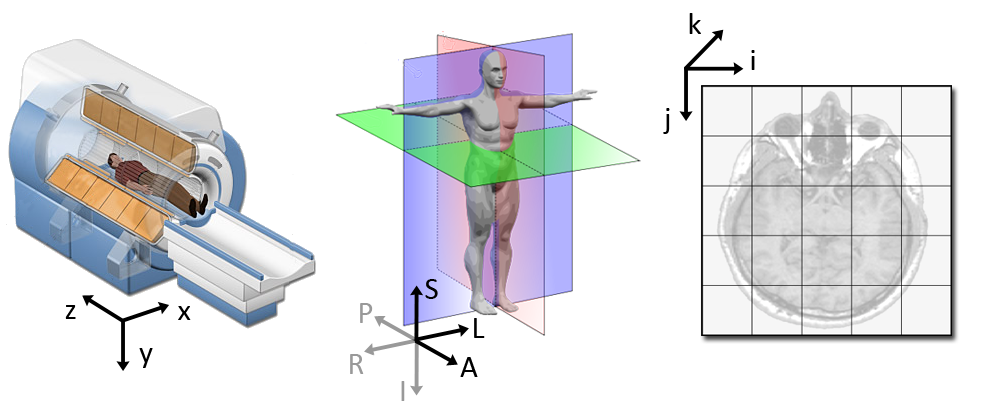
\includegraphics{Coordinate_sytems.png}
		\bicaption[CT扫描仪坐标系,人体坐标系和DICOM图像坐标系对应关系]
			{CT扫描仪坐标系,人体坐标系和DICOM图像坐标系对应关系\parencite{ctcoordinatesys2022, adaloglou2020dicomcoordinates}}
			{CT scanner, human body and DICOM imaging coordinates}
		\label{fig:coordinate}
	\end{figure}
	这样,分割出来的支气管气道树三维模型其每一个体素(Voxel)就具有精确的坐标位置信息,就可以计算出支气管管腔的中心线位置。
	
	导管机器人就是沿着管腔中心线的路径移动,导航至靶标位置。目前,美国Intuitive Surgical Company已经开发出肺部导管机器人ION,并投入了临床应用。
	\begin{figure}[!htp]
		\centering
		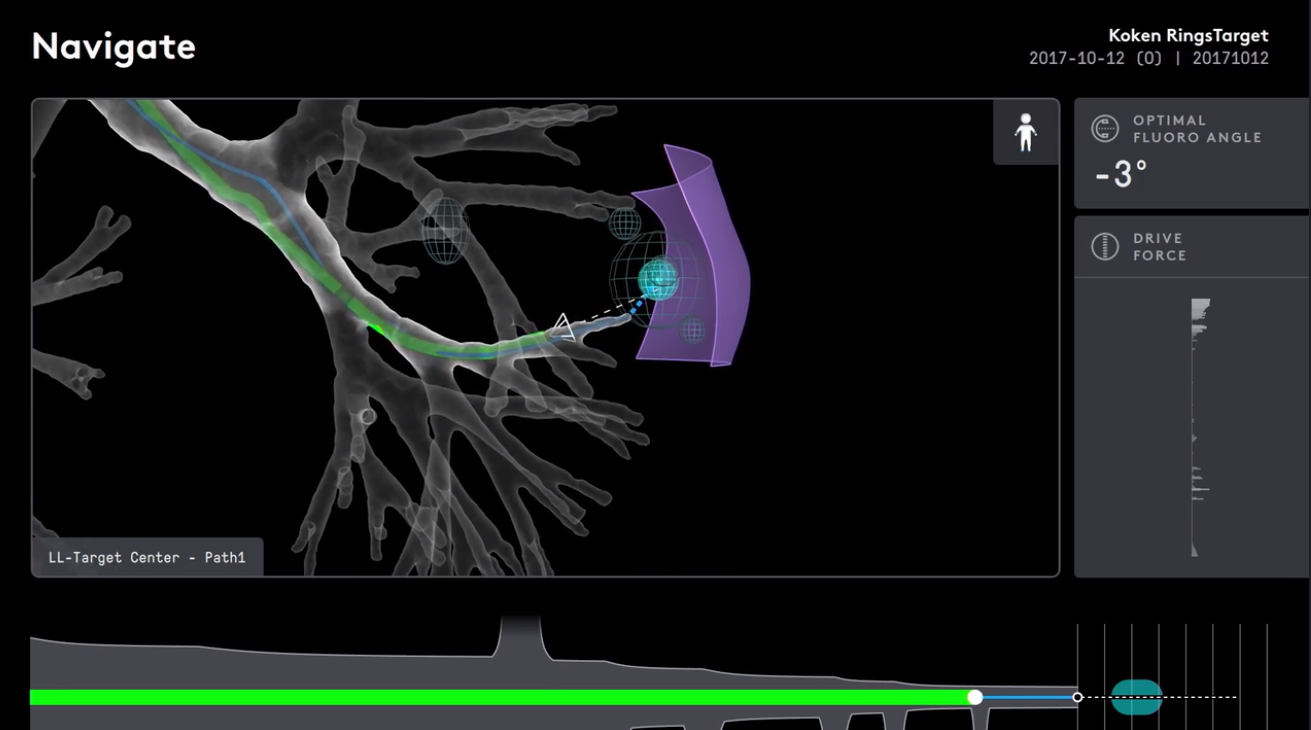
\includegraphics[width=0.45 \textwidth]{ION_robot_navigating}
		\hspace{2mm}
		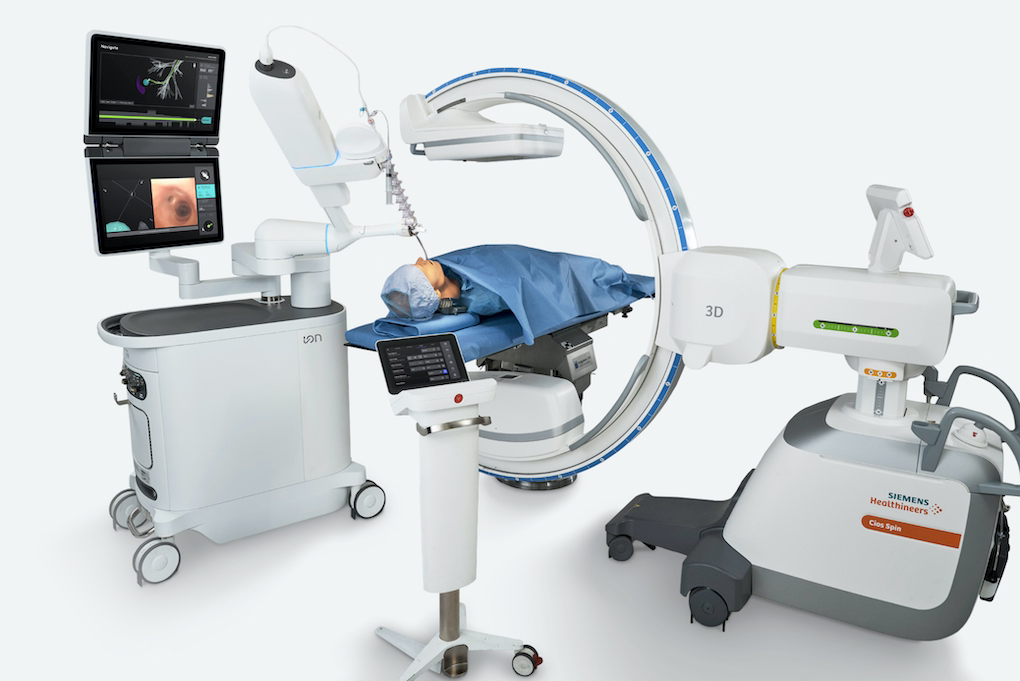
\includegraphics[width=0.45 \textwidth]{ION_bronchoscopy_robot.jpg}
		\bicaption[ION肺部导管机器人]
			{ION肺部导管机器人\parencite{ionrobot2021}}
			{ION bronchoscopy robot}
		\label{fig:ION_robot}
	\end{figure}
	
	作者所在的工作单位正在开发国产的肺部导管机器人,已经完成全国首例机器人辅助经支气管镜肺结节活检手术。
	
	当然导管手术机器人除了依赖支气管气道树三维模型导航,还需要辅助术中实时定位、支气管镜视觉导航的技术。
	
	
	\item {\heiti 智慧医疗辅助诊断}
	基于CT扫描图像的医疗图像分割需要高质量的标注数据,这很大程度上依赖经验丰富的临床医生/专家的专业知识。 为了减轻临床医生的标注压力和负担,同时亦为了减少误诊和漏诊
	的情况发生,医疗图像分割技术在医学辅助诊断上已经获得越来越多的应用。 具体到支气管气道树分割技术上,已经被用来辅助诊断一些慢性阻塞性肺部疾病COPD, 支气管扩张和肺气肿
	等一些肺部疾病。 随着AI图像分割技术的不断的进步,可以辅助临床医生更准确更高效地诊断疾病,逐渐达成智慧医疗,提高医疗技术水平和能力。
\end{itemize}



\section{研究现状和发展趋势}


图像分割技术已经发展很多年,从过去十年的发展来看,图像分割技术的发展经历了传统的图像分割方法和基于深度学习的分割方法2个阶段。传统的图像分割方法产生了一些比较经典的算法,
诸如基于阈值的最大类间方差Otsu方法\cite{otsu1979threshold},基于聚类的K-Means算法\cite{macqueen1965some}等。而随着近年来深度学习的发展,深度学习应用于图像分割
则是涌现了大量优秀的分割方法。Jonathan Long等人\cite{long2015fully}首次提出的全卷积网络(Fully Convolution Neural Network, FCN), 最经典的当属Olaf Ronneberger等人\cite{ronneberger2015u}提出的UNet结构,以及在UNet基础上改进提出的V-Net\cite{milletari2016v}结构模型、U-Net++\cite{zhou2019unet++}
结构模型,还有针对医疗影像这类三维体数据的分割模型3D UNet结构\cite{cciccek20163d},诸如这些基于深度学习的图像分割模型,其性能、精度、鲁棒性等指标都在不断进步,发展非常活跃。

下面分别介绍传统的图像分割方法、基于深度学习的图像分割方法和具体针对肺部支气管气道树的分割方法,了解他们的基本思想和发展趋势。

	\subsection{传统的图像分割方法}
	
	传统图像分割的方法是根据图像特征设计相应的算法对每个像素点进行分类,这些图像的特征包括颜色、纹理、亮度和形状等,其本质是根据特定标准确定一个合理的阈值,将每一个
	像素点与此阈值比较,以确定每一个像素点的分类。综合分析传统的图像分割方法,我们可以总结出如下的划分:
	\begin{enumerate}
		\item 阈值法
		
		阈值法是根据图像的灰度特征信息进行与阈值比较的计算。对欲分割的图像设定一个或多个(不同)的阈值,然后将图像上的每一个像素点与阈值进行比较,得到每个像素点所属的
		类别。这方面主要的工作有Sauvola法\cite{sauvola2000adaptive}、最大类间方差Otsu法\cite{otsu1979threshold}等。医疗图像(DICOM格式\cite{mustra2008overview})都是典型的灰度图\ref{fig:medical_image}。
		\begin{figure}[!htp]
			\centering
			\begin{subfigure}{\textwidth}
				\centering
				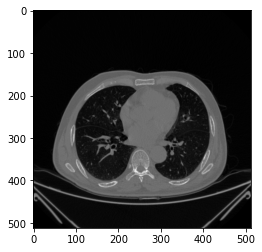
\includegraphics[scale=0.8]{DICOM image(axial view)}
				\caption{轴向面视图}
			\end{subfigure}
			
			\vspace{2mm}
			
			\begin{subfigure}{\textwidth}
				\centering
				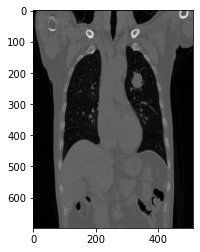
\includegraphics[scale=0.8]{DICOM image(coronal view)}
				\caption{冠状面视图}
			\end{subfigure}
			\bicaption[医疗图像(DICOM格式的灰度图)]
				{医疗图像(DICOM格式的灰度图)}
				{Medical image in DICOM format}
			\label{fig:medical_image}
		\end{figure}
		
		\item 区域法
		
		区域法是根据像素的灰度和纹理信息,以区域一致性规则进行分割。其包括:区域生长法、区域分裂、区域合并法。区域生长法通过指定一个种子点,向生长区域不断地添加满足
		约束条件的新的像素,直到填满或无法再添加。这些新添加进来的像素即属于一个类别,在不同的生长区域的像素从属于不同的类别。区域法初始形式简单,计算速度也快,它比较
		适合灰度均匀的图像分割。
		
		\item 聚类法
		
		聚类方法则根据像素间的特征相似程度进行迭代式的分类,将特征值相近的一组像素归为一个类别,然后计算这一组像素的中心位置。通过不断更新迭代直到完成所有像素的分类。
		这种方法的代表性工作便是K-Means算法\cite{macqueen1965some},聚类法使同类像素样本尽可能相近,而异类像素样本则拉大差异。聚类法的实现较为简单,但缺点就是
		对噪声很敏感,稍微不同的聚类中心和类别选择等因素都会导致分割结果差异,鲁棒性较差。
		
		\item 图论法
		
		图论法源于聚类的分割方法,它是将图像转换成带权重的无向图,将无向图划分为各种子图,使每个子图内部保持最大相似性,而子图之间则是差异尽可能大,每个子图代表
		一个类别。相关的图论分割方法就有归一化图分割、最小图分割、迭代式图分割等。
	\end{enumerate}
	
	\subsection{基于深度学习的图像分割方法}
	
	传统的图像分割方法围绕着图像的某一个具体特征进行精心挑选,设计与之匹配的算法,不具备广泛性和普遍性。 对于医疗的CT扫描图像,如前文图\ref{fig:medical_image}
	所述的都是对比度小的灰度图,传统的图像分割方法对于医疗图像不再适合。
	
	近年来随着深度学习技术在计算机视觉领域的应用,飞速发展并取得显著的进步。 基于深度卷积神经网络的语义分割方法对图像中的所有像素进行精确预测,预测像素属于哪一个类别
	的概率,赋予其标签,通过不断地迭代,从而分割出来图像。自美国加州大学UC Berkeley的Jonathan Long等人\cite{long2015fully}首次提出端到端、像素到像素的全卷积网络
	Fully Convolution Networks for Semantic Segmentation,取得的图像分割效果明显超过以往传统的图像分割法。以此为标志,打开了深度学习在图像分割领域应用的新通
	道。全卷积网络FCN由多个卷积层和池化层组合而成,学习图像中每个像素的语义信息,最后生成像素级的类别概率预测图。
	\begin{figure}[!htp]
		\centering
		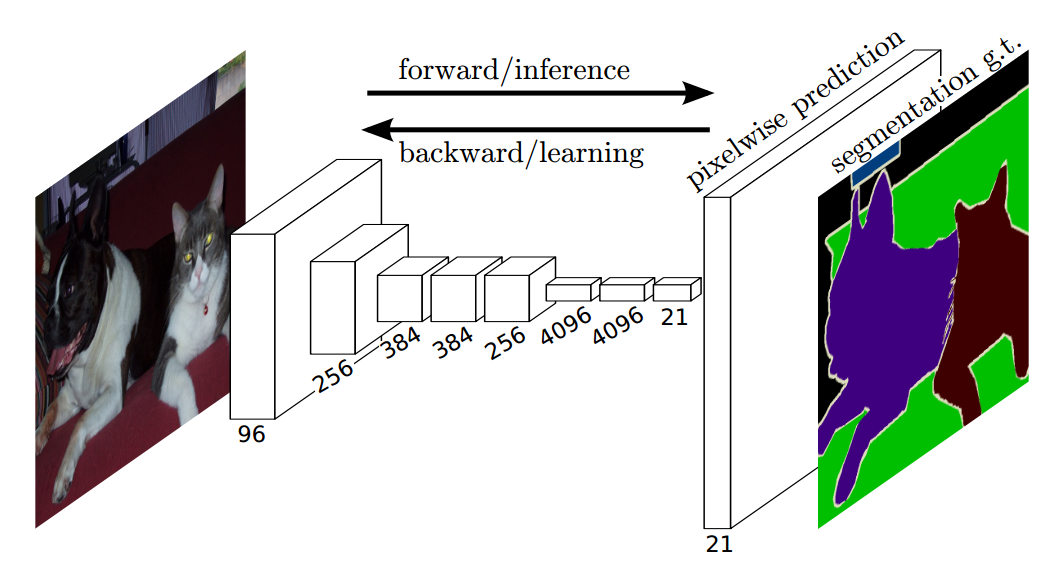
\includegraphics[width = 0.7 \textwidth]{FCN网络的结构}
		\bicaption[FCN网络的结构]
			{FCN网络的结构\cite{long2015fully}}
			{The structure of Fully Convolution Networks}
		\label{fig:FCN}
	\end{figure}
	
	但由于下采样路径上图像分辨率显著被降低,使得最后的预测结果比较粗糙。正如图\ref{fig:FCN}中分割结果只能看到2个物体的轮廓,无法看出是一只猫或是一只狗。在此基础上,
	Hyeonwoo Noh等人\cite{Noh2015LearningDN}添加进去了上采样路径,亦即反卷积Deconvolution,同步加入反池化Unpooling,将图像分辨率逐步恢复到原来的分辨率。
	\begin{figure}[!htp]
		\centering
		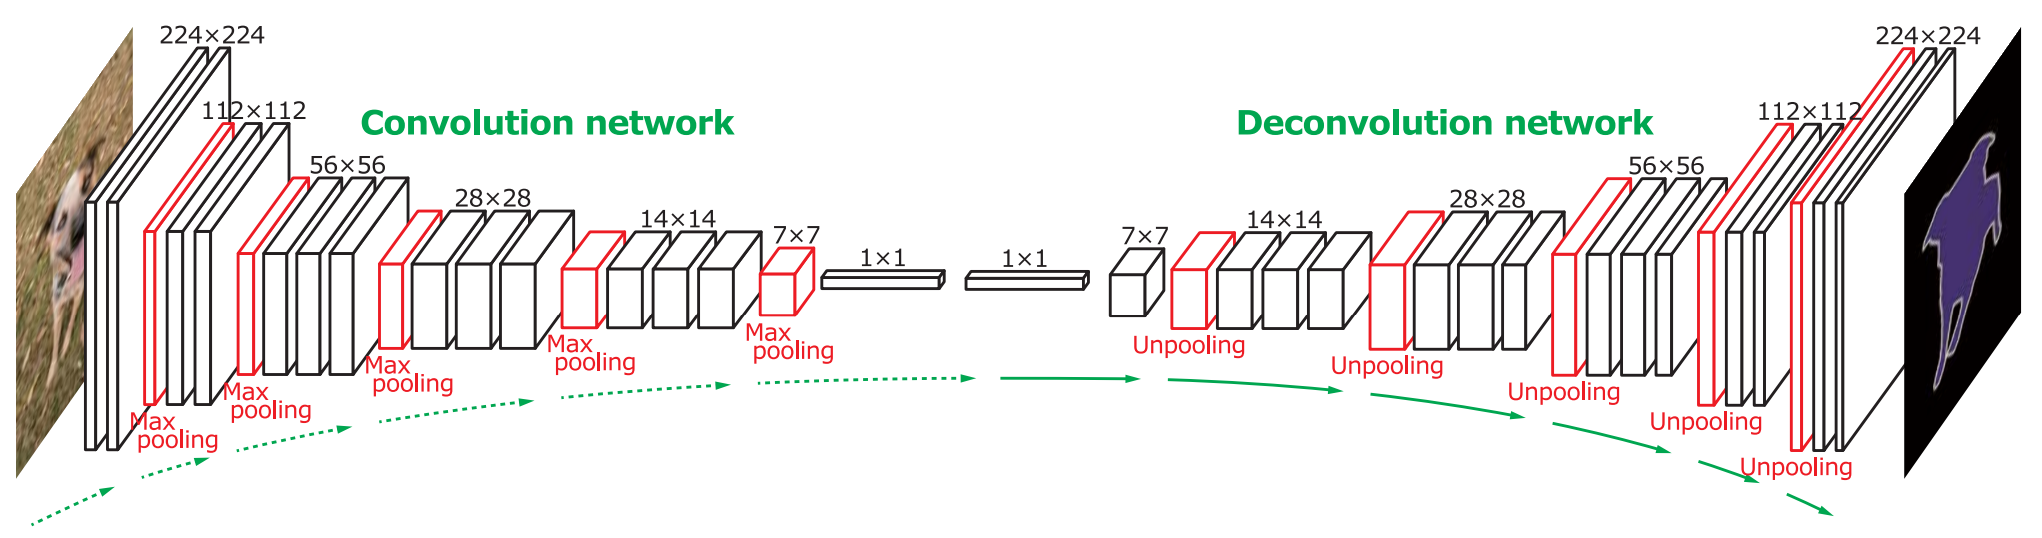
\includegraphics[width = 0.7 \textwidth]{Convolution_and_Deconvolution_network}
		\bicaption[卷积下采样路径 vs. 反卷积上采样路径]
			{卷积下采样路径 vs. 反卷积上采样路径\cite{Noh2015LearningDN}}
			{Convolutuion in down-samping path vs. Deconvolution in up-samping path}
		\label{fig:conv_deconv}
	\end{figure}
	\begin{figure}[!htp]
		\centering
		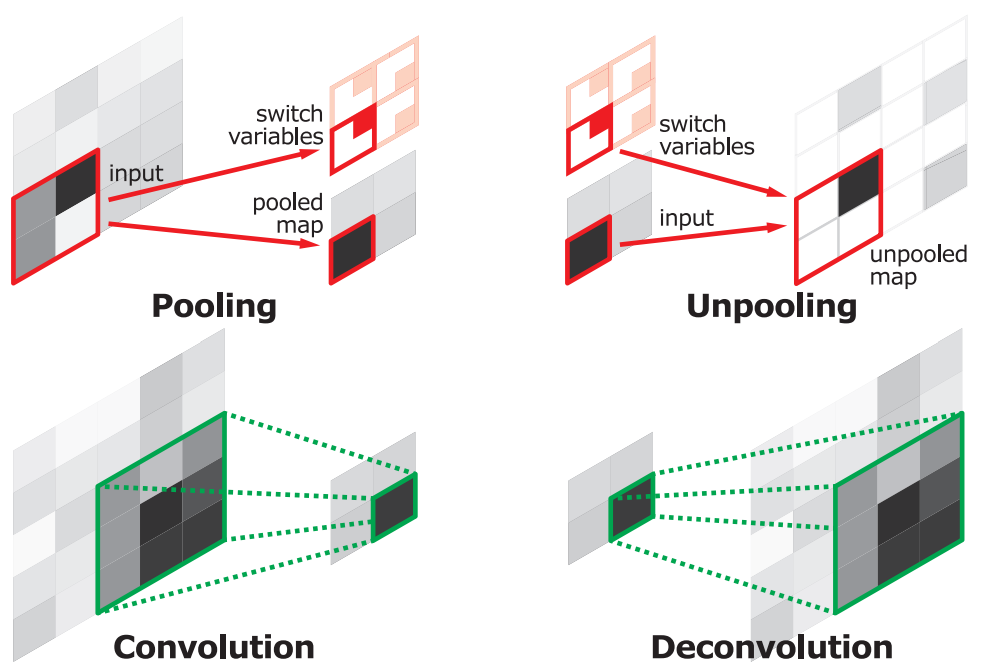
\includegraphics[width=0.6 \textwidth]{Deconvolution_and_unpooling_operations}
		\bicaption[卷积与反卷积,池化与反池化的操作]
			{卷积与翻卷积、池化与反池化的操作\cite{Noh2015LearningDN}}
			{The operations of convolution/deconvolution, and pooling/unpooling}
		\label{fig:conv_deconv_pooling_unpooling}
	\end{figure}
	
	图\ref{fig:conv_deconv}中的Convolution network与Deconvolution network也分别被成为编码器Encoder与解码器Decoder,这两条对称路径构成了Encoder-Deconder
	图像语义分割网络架构。
	
	后来,Olaf Ronneberger等人\cite{ronneberger2015u}则进一步改进,保留下采样路径用于提取深度特征信息,而在上采样路径则加入了跳跃连接,将下采样获取的深度特征信息
	跳跃过来与上采样拼接起来,实现特征图融合。这就是经典的U-Net网络结构。U-Net网络实现了更精细的图像语义分割结果。
	
	\begin{figure}[!htp]
		\centering
		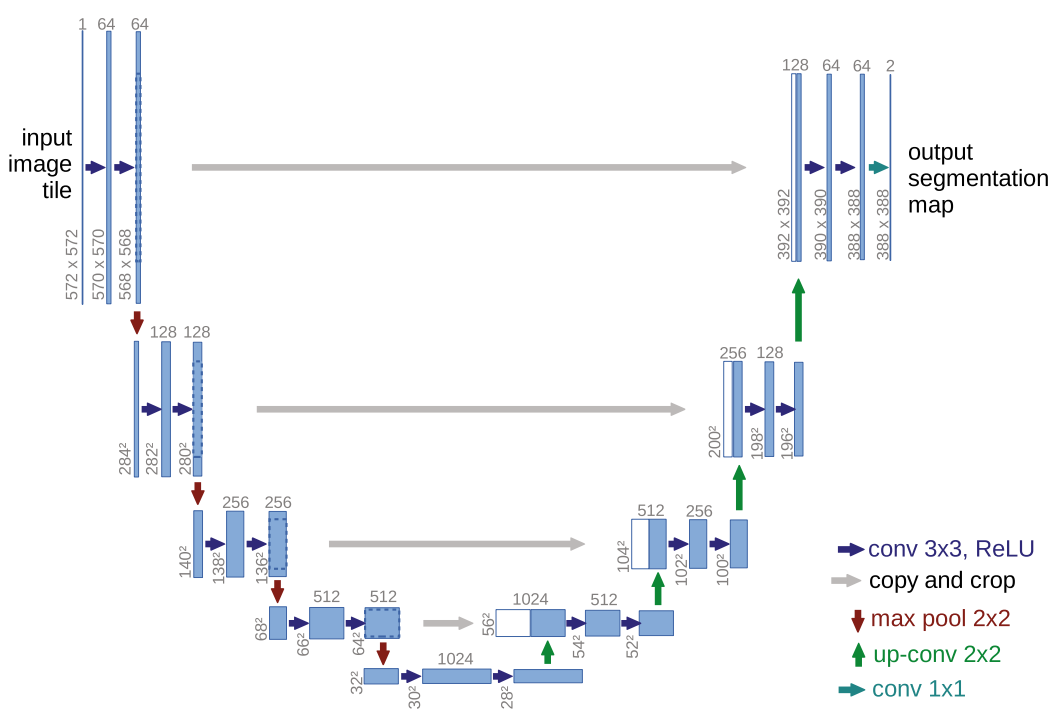
\includegraphics[width=0.7\textwidth]{UNet_architecture}
		\bicaption[经典的图像分割U-Net网络结构]
			{经典的图像分割U-Net网络结构\cite{ronneberger2015u}}
			{The classic U-Net architecture for image segmentation}
		\label{fig:UNet}
	\end{figure}
	
	U-Net网络目前已成为医疗图像分割任务的基础网络,有很多研究人员在U-Net基础上改进,应用在医疗图像的分割。比如肝脏、肺癌结节、乳腺肿块等不同的疾病。Li Xiaomeng等人
	\cite{Li2017HDenseUNetHD}提出一种基于U-Net混合式的稠密连接的新型网络结构H-DenseUNet用于肝癌的医疗CT图像的分割。它将UNet的保留低卷积层的细节特征,UNet网络
	越来越深的层次增加了训练的长耗时,而H-DenseUNet又可以解决这些深层网络的长耗时训练困难。
	
	医疗CT扫描图像基本上都是三维体数据,基于此又引申发展出3D CNN, Jose Dolz等人\cite{Dolze3DFCN}就提出了3D Fully convolutional networks, {\"O}zg{\"u}n {\c{C}}i{\c{c}}ek等人\cite{cciccek20163d}则提出3D UNet用于稠密的体数据分割。如此众多的分割网络,各个作者在UNet的基础上加上自己的创新,形成一个个独具特色的新型
	网络结构。那有没有一种广泛通用的网络来做图像分割呢? Mathias Perslev等人\cite{PerslevGeneralUNetFusion}就提出了这样的一个想法和实施方案
	One Network to segment them all一种通用	的轻量级的网络结构来精确分割3D图像。它是在UNet网络之后再加上一个Fusion model实现的。
	\begin{figure}[!htp]
		\centering
		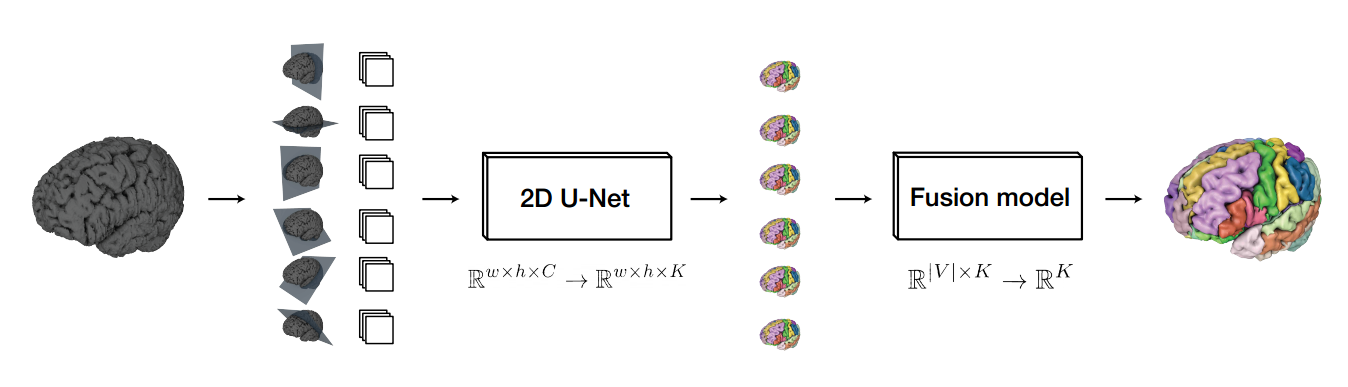
\includegraphics[width=0.8\textwidth]{Genral_UNet}
		\bicaption[一种通用的轻量化的UNet网络]
			{一种通用的轻量化的UNet网络\cite{PerslevGeneralUNetFusion}}
			{A general, lightweight UNet to segment them all}
		\label{fig:Genral_UNet}
	\end{figure}
	
	最近三年,新冠肺炎疫情肆虐全球,为了抗击疫情,许多研究人员的兴趣都被COVID-19吸引过去,争相研究感染了新冠病毒的肺部CT影像,以期帮助医疗专家、临床医生理解被感染
	后的肺部症状,预测是否感染了新冠肺炎。Zahid Ullah等人\cite{Ullah2023DenselyAM}提出一种稠密型注意力机制的网络来检测COVID-19的感染情况. 其网络结构(图
	\ref{fig:COVID19})在卷积层后插入通道注意力层和稠密区块层,使其聚焦于感兴趣的感染区域,从而高效地检测出感染情况。
	\begin{figure}[!htp]
		\centering
		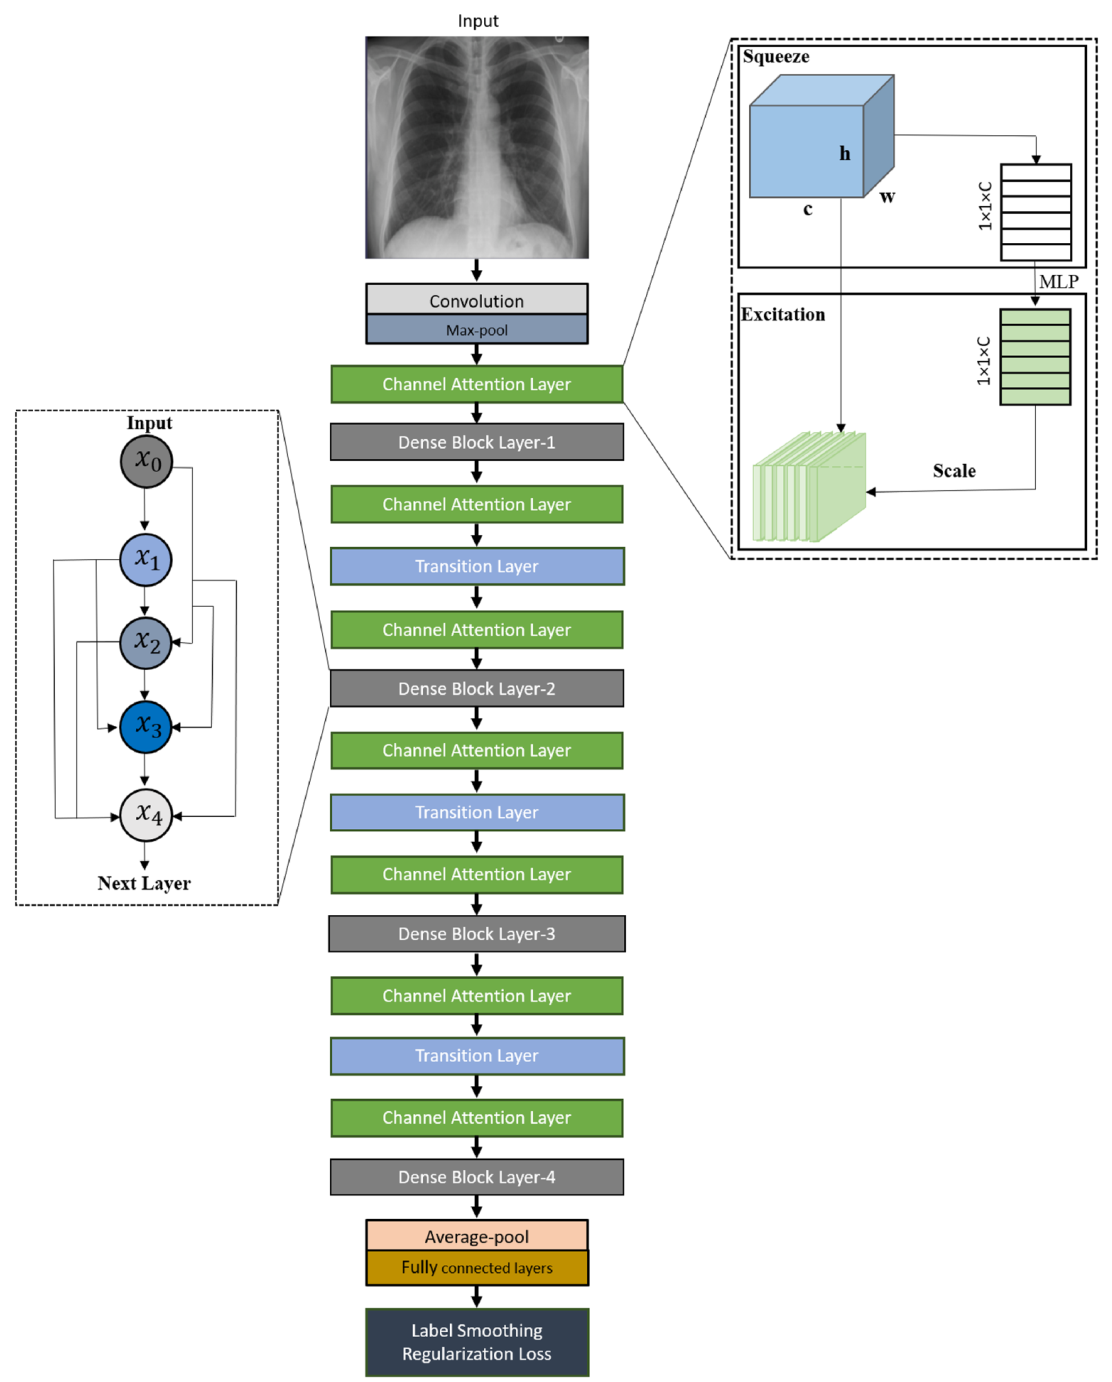
\includegraphics[width=0.5\textwidth]{Densely_attention_mechanism_based_network}
		\bicaption[稠密型注意力机制网络用来检测 COVID-19的感染情况]
			{稠密型注意力机制网络用来检测 COVID-19的感染情况\cite{Ullah2023DenselyAM}}
			{Densely attention mechanism network to detect the COVID-19 infection}
		\label{fig:COVID19}
	\end{figure}
	通过跟正常肺部影像和普通肺炎所造成阴影区域对比,比较明确地指出COVID-19感染区域(图\ref{fig:COVID19_detection}中COVID-19一栏所高亮显示的),展现给临床医生,辅助诊断是否感染新冠肺炎。
	\begin{figure}[!htp]
		\centering
		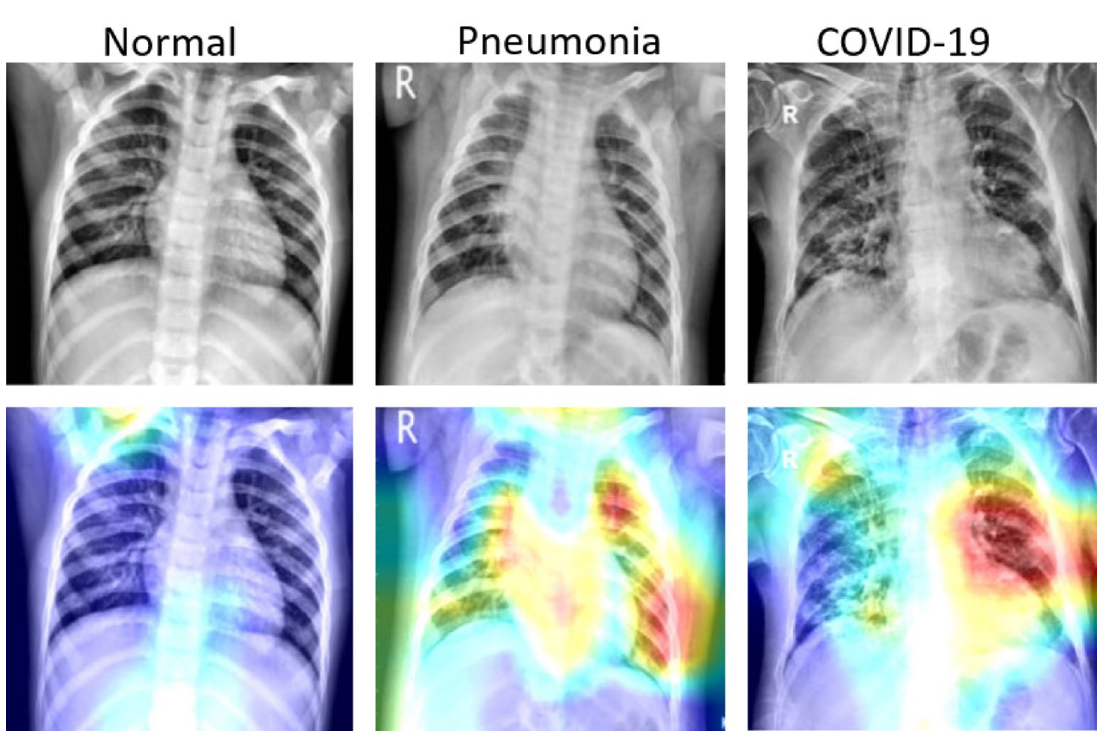
\includegraphics[width=0.8\textwidth]{Detect_COVID19_infection}
		\bicaption[对比正常肺部阴影、普通肺炎和COVID-19新冠肺炎的阴影,突出新冠肺炎感染区域]
			{对比正常肺部阴影、普通肺炎和COVID-19新冠肺炎的阴影,突出新冠肺炎感染区域\cite{Ullah2023DenselyAM}}
			{Highlight the COVID-19 infection area by comparing with normal and pneumonia}
		\label{fig:COVID19_detection}
	\end{figure}
	
	最新的进展是,随着NLP的Transformer模型\cite{Devlin2019BERTPO, NIPS2017Attention}取得成功后,NVIDIA的Ali Hatamizadeh和Vanderbilt Unversity的Yucheng Tang
	等人\cite{unetr}受此启发,率先将Transformer引入3D medical image segmentation中来,提出了UNETR网络结构(见图\ref{fig:UNETR}所示),实现了State-of-the-art (SOTA)医疗图像
	分割性能新记录。
	\begin{figure}[!htp]
		\centering
		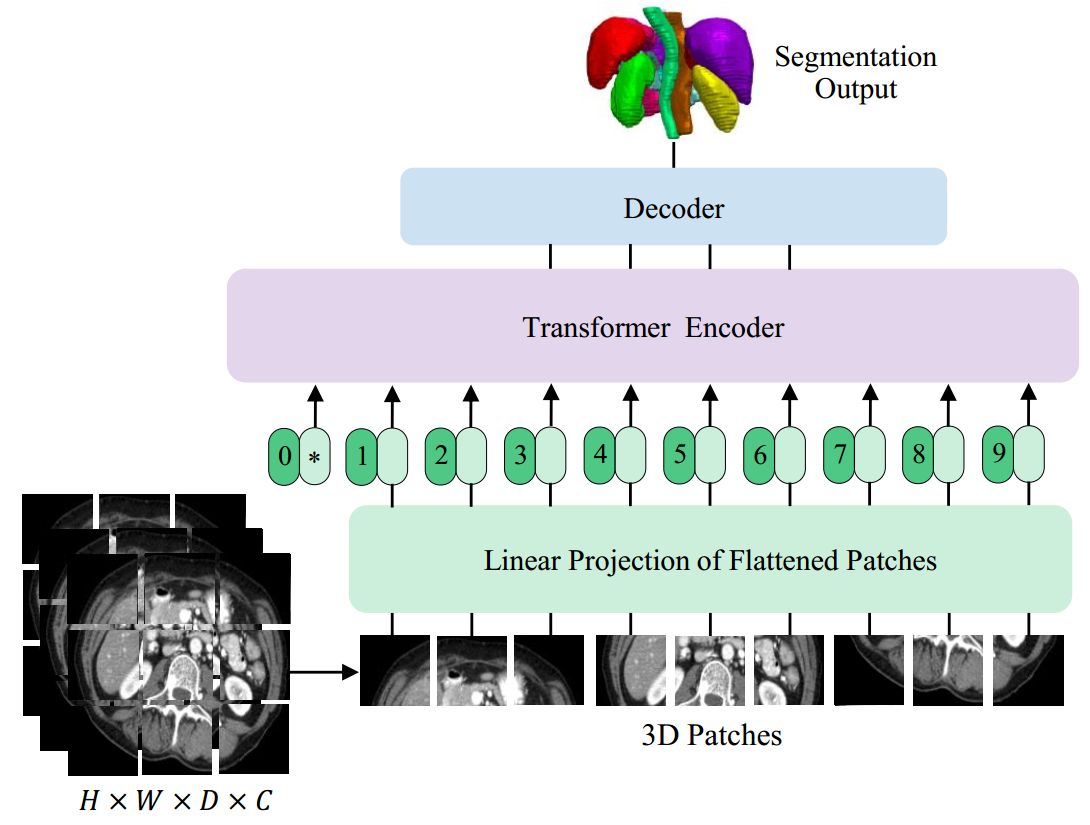
\includegraphics[width=0.6\textwidth]{Overview_of_UNETR}
		\bicaption[UNET网络基本结构]
			{UNETR网络基本结构\cite{unetr}}
			{The basic structure of UNETR network}
		\label{fig:UNETR}
	\end{figure}
	
	综上所述,基于深度学习的医疗图像分割技术发展非常活跃,研究进展迅速,进步巨大。
	
	
	
	\subsection{针对肺部支气管气道树的医疗图像分割方法}
	对于肺部CT图像的分割,卷积神经网络CNN早就应用在上面了。最知名的LUng Nodule Analysis 2016大挑战竞赛要求参赛选手分割出Lung CT图像的肺结节,判断肺结节是
	良性的还是恶性的,从而筛选出肺癌疑似患者,进行早期预防和针对性治疗。从LUNA16大挑战竞赛里诞生了两个具有重要影响力的公开数据集LUNA和LIDC-IDRI。 类似于LUNA
	大挑战竞赛,针对肺部支气管气道树的分割也有一个比较著名的EXtraction of Ariways from CT 2009 (EXACT'09)竞赛项目。Marleen de Bruijne等
	人\cite{Lo2012ExtractionOA}在2009年发起了EXACT'09这个竞赛项目,其研究目标就是提供一个公开通用的数据集,鼓励参赛选手开发出创新性算法,从胸部CT扫描图像中提取出
	支气管气道树,评比参赛选手门提交的算法。
	
	自EXACT'09大挑战竞赛的激励后涌现了大量的研究成果, Zhao Tianyi等人\cite{Zhao2019BronchusSA}开发出来一个两阶段2D + 3D的神经网络和一个基于线性规划的气道
	分割跟踪算法




























































\chapter{简介}

这是 \sjtuthesis 的示例文档,基本上覆盖了模板中所有格式的设置。建议大家在使用模
板之前,除了阅读《\sjtuthesis\ 使用文档》,这个示例文档也最好能看一看。

\section{二级标题}

\subsection{三级标题}

\subsubsection{四级标题}

Lorem ipsum dolor sit amet, consectetur adipiscing elit, sed do eiusmod tempor
incididunt ut labore et dolore magna aliqua. Ut enim ad minim veniam, quis
nostrud exercitation ullamco laboris nisi ut aliquip ex ea commodo consequat.
Duis aute irure dolor in reprehenderit in voluptate velit esse cillum dolore eu
fugiat nulla pariatur. Excepteur sint occaecat cupidatat non proident, sunt in
culpa qui officia deserunt mollit anim id est laborum.

\section{脚注}

Lorem ipsum dolor sit amet, consectetur adipiscing elit, sed do eiusmod tempor
incididunt ut labore et dolore magna aliqua. \footnote{Ut enim ad minim veniam,
quis nostrud exercitation ullamco laboris nisi ut aliquip ex ea commodo
consequat. Duis aute irure dolor in reprehenderit in voluptate velit esse cillum
dolore eu fugiat nulla pariatur.}

\section{字体}


上海交通大学是我国历史最悠久的高等学府之一,是教育部直属、教育部与上海市共建的全
国重点大学,是国家“七五”、“八五”重点建设和“211 工程”、“985 工程”的首批建
设高校。经过 115 年的不懈努力,上海交通大学已经成为一所“综合性、研究型、国际化”
的国内一流、国际知名大学,并正在向世界一流大学稳步迈进。 

{\songti 十九世纪末,甲午战败,民族危难。中国近代著名实业家、教育家盛宣怀和一批
  有识之士秉持“自强首在储才,储才必先兴学”的信念,于 1896 年在上海创办了交通大
  学的前身——南洋公学。建校伊始,学校即坚持“求实学,务实业”的宗旨,以培养“第
  一等人才”为教育目标,精勤进取,笃行不倦,在二十世纪二三十年代已成为国内著名的
  高等学府,被誉为“东方MIT”。抗战时期,广大师生历尽艰难,移转租界,内迁重庆,
  坚持办学,不少学生投笔从戎,浴血沙场。解放前夕,广大师生积极投身民主革命,学校
  被誉为“民主堡垒”。}

{\heiti 新中国成立初期,为配合国家经济建设的需要,学校调整出相当一部分优势专业、
  师资设备,支持国内兄弟院校的发展。五十年代中期,学校又响应国家建设大西北的号
  召,根据国务院决定,部分迁往西安,分为交通大学上海部分和西安部分。1959 年 3月
  两部分同时被列为全国重点大学,7 月经国务院批准分别独立建制,交通大学上海部分启
  用“上海交通大学”校名。历经西迁、两地办学、独立办学等变迁,为构建新中国的高等
  教育体系,促进社会主义建设做出了重要贡献。六七十年代,学校先后归属国防科工委和
  六机部领导,积极投身国防人才培养和国防科研,为“两弹一星”和国防现代化做出了
  巨大贡献。}

{\kaishu 改革开放以来,学校以“敢为天下先”的精神,大胆推进改革:率先组成教授代
  表团访问美国,率先实行校内管理体制改革,率先接受海外友人巨资捐赠等,有力地推动
  了学校的教学科研改革。1984 年,邓小平同志亲切接见了学校领导和师生代表,对学校
  的各项改革给予了充分肯定。在国家和上海市的大力支持下,学校以“上水平、创一流”
  为目标,以学科建设为龙头,先后恢复和兴建了理科、管理学科、生命学科、法学和人文
  学科等。1999 年,上海农学院并入;2005 年,与上海第二医科大学强强合并。至此,学
  校完成了综合性大学的学科布局。近年来,通过国家“985 工程”和“211 工程”的建
  设,学校高层次人才日渐汇聚,科研实力快速提升,实现了向研究型大学的转变。与此同
  时,学校通过与美国密西根大学等世界一流大学的合作办学,实施国际化战略取得重要突
  破。1985 年开始闵行校区建设,历经 20 多年,已基本建设成设施完善,环境优美的现
  代化大学校园,并已完成了办学重心向闵行校区的转移。学校现有徐汇、闵行、法华、七
  宝和重庆南路(卢湾)5 个校区,总占地面积 4840 亩。通过一系列的改革和建设,学校
  的各项办学指标大幅度上升,实现了跨越式发展,整体实力显著增强,为建设世界一流大
  学奠定了坚实的基础。}

{\ifcsname fangsong\endcsname\fangsong\else[无 \cs{fangsong} 字体。]\fi 交通大学
  始终把人才培养作为办学的根本任务。一百多年来,学校为国家和社会培养了 20余万各
  类优秀人才,包括一批杰出的政治家、科学家、社会活动家、实业家、工程技术专家和医
  学专家,如江泽民、陆定一、丁关根、汪道涵、钱学森、吴文俊、徐光宪、张光斗、黄炎
  培、邵力子、李叔同、蔡锷、邹韬奋、陈敏章、王振义、陈竺等。在中国科学院、中国工
  程院院士中,有 200 余位交大校友;在国家 23 位“两弹一星”功臣中,有 6 位交大校
  友;在 18 位国家最高科学技术奖获得者中,有 3 位来自交大。交大创造了中国近现代
  发展史上的诸多“第一”:中国最早的内燃机、最早的电机、最早的中文打字机等;新中国
  第一艘万吨轮、第一艘核潜艇、第一艘气垫船、第一艘水翼艇、自主设计的第一代战斗
  机、第一枚运载火箭、第一颗人造卫星、第一例心脏二尖瓣分离术、第一例成功移植同种
  原位肝手术、第一例成功抢救大面积烧伤病人手术等,都凝聚着交大师生和校友的心血智
  慧。改革开放以来,一批年轻的校友已在世界各地、各行各业崭露头角。}

{\ifcsname lishu\endcsname\lishu\else[无 \cs{lishu} 字体。]\fi 截至 2011 年 12
  月 31 日,学校共有 24 个学院 / 直属系(另有继续教育学院、技术学院和国际教育学
  院),19 个直属单位,12 家附属医院,全日制本科生 16802 人、研究生24495 人(其
  中博士研究生 5059 人);有专任教师 2979 名,其中教授 835 名;中国科学院院士 15
  名,中国工程院院士 20 名,中组部“千人计划”49 名,“长江学者”95 名,国家杰出
  青年基金获得者 80 名,国家重点基础研究发展计划(973 计划)首席科学家 24名,国
  家重大科学研究计划首席科学家 9名,国家基金委创新研究群体 6 个,教育部创新团队
  17 个。}

{\ifcsname youyuan\endcsname\youyuan\else[无 \cs{youyuan} 字体。]\fi 学校现有本
  科专业 68 个,涵盖经济学、法学、文学、理学、工学、农学、医学、管理学和艺术等九
  个学科门类;拥有国家级教学及人才培养基地 7 个,国家级校外实践教育基地 5个,国
  家级实验教学示范中心 5 个,上海市实验教学示范中心 4 个;有国家级教学团队 8个,
  上海市教学团队 15 个;有国家级教学名师 7 人,上海市教学名师 35 人;有国家级精
  品课程 46 门,上海市精品课程 117 门;有国家级双语示范课程 7 门;2001、2005 和
  2009 年,作为第一完成单位,共获得国家级教学成果 37 项、上海市教学成果 157
  项。}
